\documentclass[12pt]{ltjsarticle}
\usepackage{semi}


\begin{document}
\begin{titlepage}
  \begin{center}
  
    \vspace*{20truept}
    
    {\LARGE 2023年度 卒業論文} 
    
    \vspace*{75truept}
    
    {\Huge } %論文タイトル

    \vspace{10truept}

    {\Huge 民俗芸能育成問題における} %論文タイトル 長い場合 改行1

    \vspace{10truept}

    {\Huge 小学生向け学習教材の開発} %論文タイトル 改行2

    \vspace{85truept}
    
    {\LARGE 指導教員 須田 宇宙 准教授}
    
    \vspace{60truept}
    
    {\LARGE 千葉工業大学 情報ネットワーク学科}
    
    \vspace{15truept}
    
    {\LARGE 須田研究室}
    
    \vspace{70truept}
    
    {\LARGE 1932102 氏名 永塚 迅一 } % 氏名は消さない 学生番号 氏名 名前

    \vspace{70truept}
    
  \end{center}
  \begin{flushright}

    {\LARGE 提出日 2023年1月17日}
  
  \end{flushright}
\end{titlepage}

\newpage
\setcounter{tocdepth}{3}
\pagenumbering{roman}
\pagestyle{plain}



%目次の出力
\tableofcontents
%表目次の出力
\listoftables
%図目次の出力
\listoffigures
\newpage
\pagenumbering{arabic}
\section{緒言}

%背景

日本では古くから,神の存在を崇め,奉っていた.そのため,祭りや地域の行事,豊作の祈願などの際に,様々な芸を披露して神へ祈りを捧げていた.この芸が芸能
の発端であり,何世代にも渡って継承され,現在も披露されている芸能を伝統芸能という.

伝統芸能は,歌舞伎,能楽,文楽,古典落語などがあり,その多くは,舞や音楽,そして独特な衣装や小道具などを駆使して,人々を魅了している.

しかし,生活の多忙化や少子高齢化,若者の首都圏極集中などによって,伝統芸能の活動総人口が減っている.そのため,伝統芸能の役者の高齢化や,後継者不足
が加速しており,満足に活動することができない問題がある.


伝統芸能の中に,地域の特色が強く入り,地域ごとに伝承されている民俗芸能がある.
茨城県の民俗芸能に「女沼のささら」という獅子舞があり,ささら保存会によって保存継承されている.




%問題点
また、地元小学校の運動会では,4年生から6年生の選抜された代表児童を中心に全員参加でささらを踊る.図\ref{fig:運動会}は運動会でささらを披露している様子である.
また,運動会以外にも,6年生のささら代表児童は地域の祭りでささらを
披露する機会がある.そこでささら保存会が運動会や祭りの前に,代表児童に数回指導を行なっている.しかし,ささら保存会の人数は年々減ってきており,
代表児童に対して十分な指導ができないという問題点がある.同様に,全国の主要な伝統芸能も同じ問題をかかえていると考える.
\begin{figure}[h]
  \begin{center}
   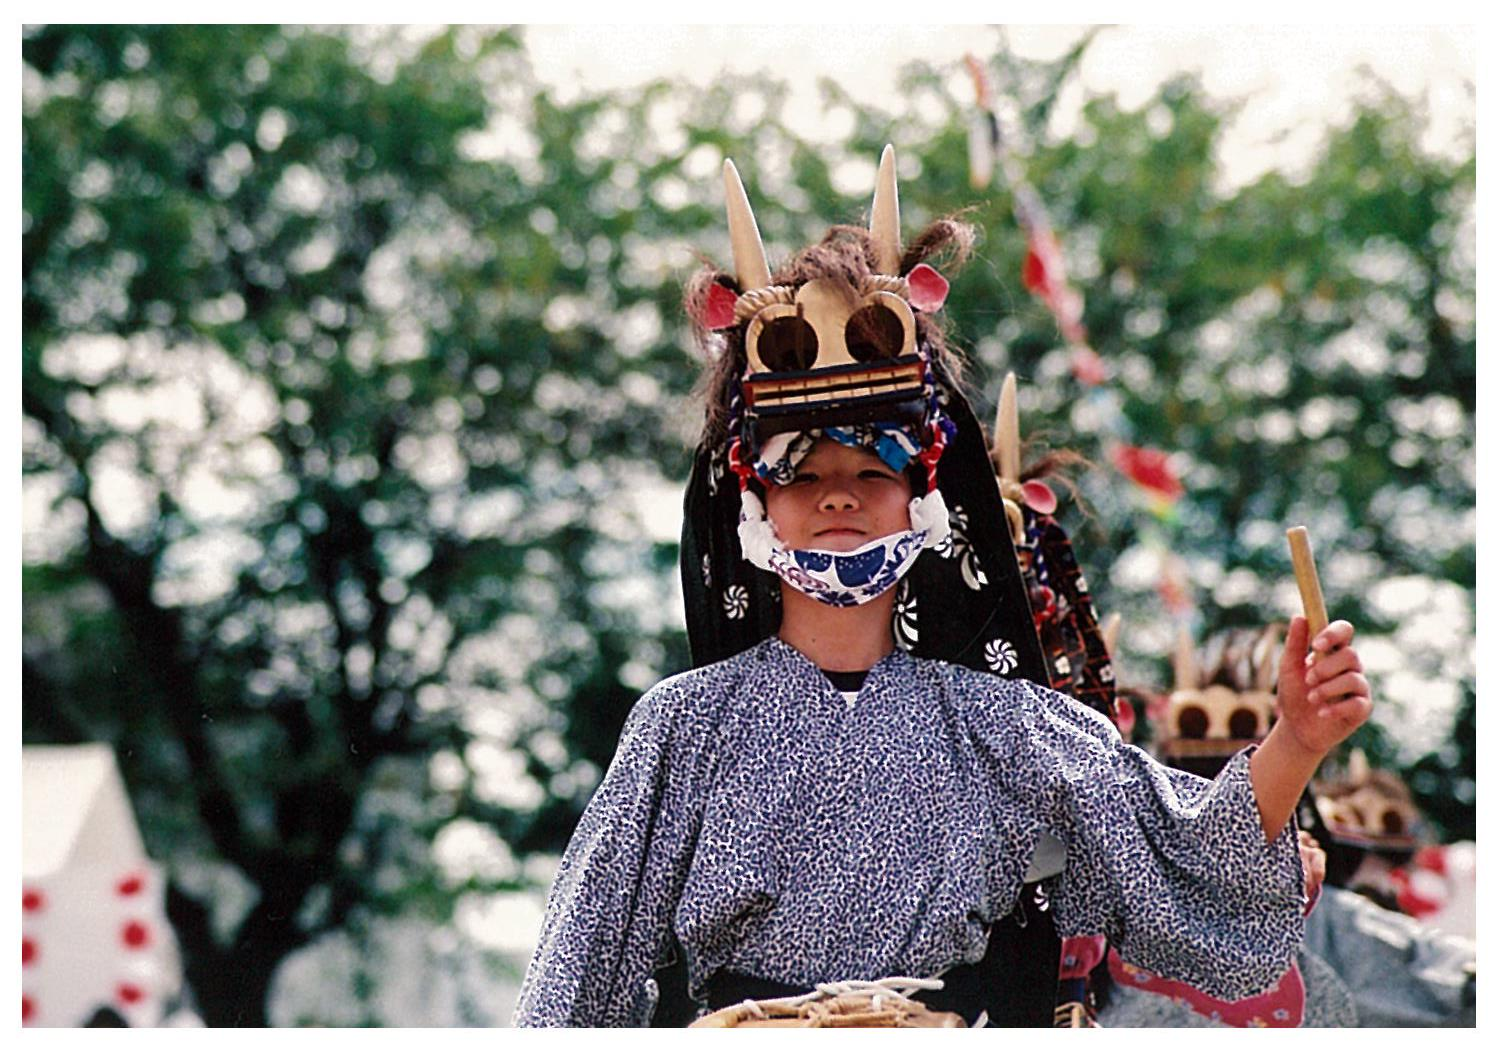
\includegraphics[clip,width=100mm]{undoukai2.jpg}
  \end{center}
   \caption{運動会でのささら発表の様子}
   \label{fig:運動会}
  \end{figure}
  
%目的
そこで本研究では,個人でささらの踊りを学習できる教材を開発し,ささら保存会の教えと併用することで代表児童に十分な踊りの情報を提供することを目的とする.
そして本教材の有用性を示し,全国の伝統芸能にも同様の教材を用いて学習することが,育成問題解決に繋がることを示したい.

\newpage
\section{日本の伝統芸能について}

\subsection{概要}

日本は古くから農業が盛んで,様々な作物を育てていた.しかし,自然災害によって,豊作ではない年もあった.そこで人々は,神に祈りを捧げ,豊作を祈願し,豊作の年には
神へ感謝の祈りを込めた.その際に,披露された芸が芸能の発端である.そして,芸能は,時代ごとの祭りや行事などで披露されていき,
大衆娯楽の一つと化して発展した.
その芸能を,人々は技を磨き,親子何世代にも渡って継承し続け,現在もなお残る芸能を伝統芸能と呼ぶ.
伝統芸能の多くは,西洋文化の影響を受ける前から日本にある文化を指し,明治時代以前に大成したものを指すことが多い.





\subsection{伝統芸能の種類}
伝統芸能には,歌舞伎,能楽,文楽,古典落語などがある.多くは,観客の前で,音楽に合わせて演劇を行い,見るものを
独自の世界観で魅了する.伝統芸能の中には,600年以上の歴史をもつものもあり,その時代の背景を題材として披露されている.


\subsubsection{歌舞伎}
歌舞伎は誕生当時から大衆娯楽の中心であり,華麗な舞を披露する演劇である.その歴史は,江戸時代の初期頃からと言われており,出雲の阿国の女性舞踊団から始まったと
されている\cite{kabuki}.
元禄時代に江戸と上方\footnote{関西}で大きく発達した.

歌舞伎は,主に「歌」「舞」「技」でなりたっており,三味線の旋律に合わせて物語を俳優が演じる.
女性の役を「女形」というが,歌舞伎では,男性が演じており,現在も続いている歌舞伎の特色である.

1965年に重要無形文化財に指定され,2008年には無形文化遺産の代表一覧表に登録された.






\subsubsection{能楽}
能楽とは,能と狂言からなる演劇である.その歴史は,仏教が伝わった6世紀半ば頃,中国から様々な芸能が伝わり,その中の散楽という芸能が
始めだと言われている.散楽が日本に浸透し,後に猿楽とし神社やお祭りで披露されるようになった\cite{nou}.

猿楽は時代の流れと共に変化し,猿楽の中の楽しさ,面白さを表現をしている演劇部分と,人の悲しさや,憤りを表現した演劇部分に分かれて,
前者を狂言,後者を能と呼ぶようになった.

1957年に重要無形文化財に指定され,2008年には無形文化遺産の代表一覧表に登録された.





\subsubsection{文楽}
文楽は日本古来の人形劇である.その歴史は,浄瑠璃という三味線音楽が発達した15世紀頃,近松門左衛門と義太夫という人物が,浄瑠璃の音楽と人形を
合わせて人形劇を作ったのが発端だと言われている\cite{bun}.

文楽は,物語を語る太夫の役,三味線を奏でる役,人形を操る役,の3役によって成り立つ.太夫の言動に合わせて三味線役が旋律を合わせ,人形遣いが
その情景を表現する.

1955年に人形浄瑠璃文楽が重要無形文化財に指定され,2008年には無形文化遺産の代表一覧表に登録された.




\subsubsection{古典落語}
古典落語は,巧みな話術で人々を笑わせる芸能である.その歴史は,戦国時代,客に笑い話を聞かせていた「おとぎ衆」と呼ばれる人々が発端だと言われている\cite{koten}.
一般に,江戸時代から昭和までの文化を題材とした落語を古典落語と呼び,それ以降から現代までの落語を新作落語と呼ぶ.

古典落語は,江戸時代の庶民の生活ぶりを題材とした話や怪談話などを寄席と呼ばれる,客に芸を披露する場所で演じていた.
座布団の上で座って滑稽な話をする際は,小道具なども巧に用いて,客を独自の世界観に引き込んでいた.

1995年に重要無形文化財に指定されている.












\subsection{伝統芸能の問題点}
日本独自の文化であり,先祖代々受け継がれてきた伝統芸能であるが,現在では高齢化と後継者不足の問題がある.

伝統芸能の主要な歌舞伎では,芸を代々継承している家元だけでは後継者が足りず,日本芸術文化振興会は一般から人を集め育成を行っている.
しかし,近年は一般からの志願者数が少なく,歌舞伎俳優は2019年度以降5人以下と低迷している\cite{kamon}.



地域においても,問題がある.

伝統芸能の中には,地域の特色が強く入り,地域ごとに伝承されている民俗芸能がある.
岩手県の北上市は100を超える民俗団体があり,民俗芸能が盛んな市である.北上市は2018年に
北上市民俗芸能団体連合会加盟団体アンケ―トを加盟47団体を対象に実施した\cite{sa2}.その結果,図\ref{fig:図3}では,36団体が後継者不足であった.
また,15団体が指導者の高齢化であり,継続するためには,若手の参入が必須である.
\vskip\baselineskip
\begin{figure}[h]
\begin{center}
 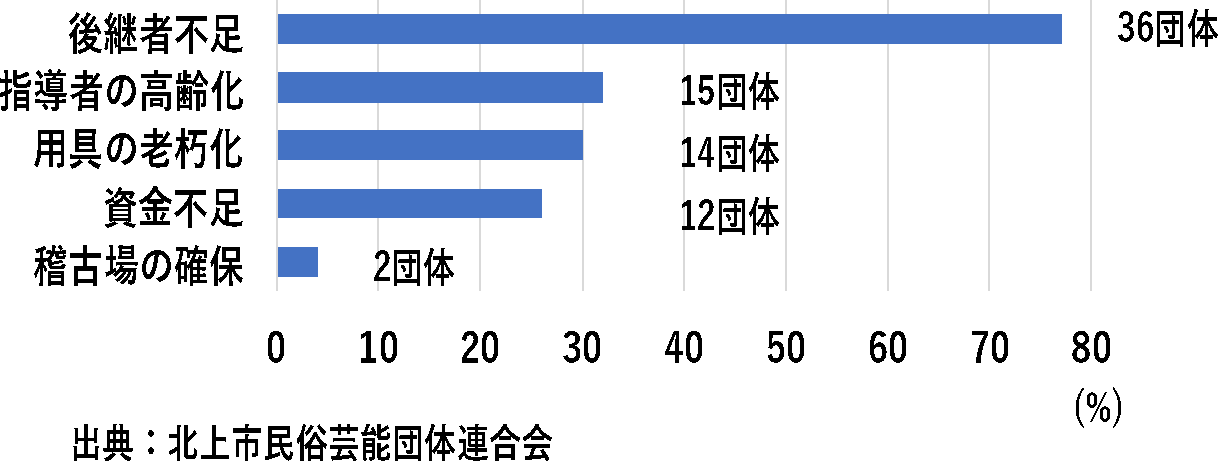
\includegraphics[clip,width=100mm]{figures/kigagami.pdf}
\end{center}
 \caption{各団体の運営におけるなやみ}
 \label{fig:図3}
\end{figure}






上記のように全国各地で伝統芸能や民俗芸能の後継者が不足している.そのため,現在伝統芸能を継承している人達で活動する必要が
あるため,内部で高齢化が進んでしまう.そのことによって,技を後世に伝えることができず,衰退の一途をたどっている現状がある.








\clearpage
\section{女沼のささら}
\subsection{概要}
女沼のささらは,地元の女沼地区に伝わる民俗芸能の一つである.「前獅子」\footnote{「前獅子」は「太夫獅子」ともいう}「女獅子」「後獅子」の「3人立ち」からなり,
腹には小太鼓を抱き,両手に持ったバチで叩きながら舞う。前,後獅子は紺,女獅子は赤の上着に袴を身に着け,草履をはいている.舞っている様子を図\ref{fig:図4}に示す.
獅子の他には,獅子が舞う際に笛を奏でている笛担当が数名いる.
\vskip\baselineskip
\begin{figure}[h]
\begin{center}
 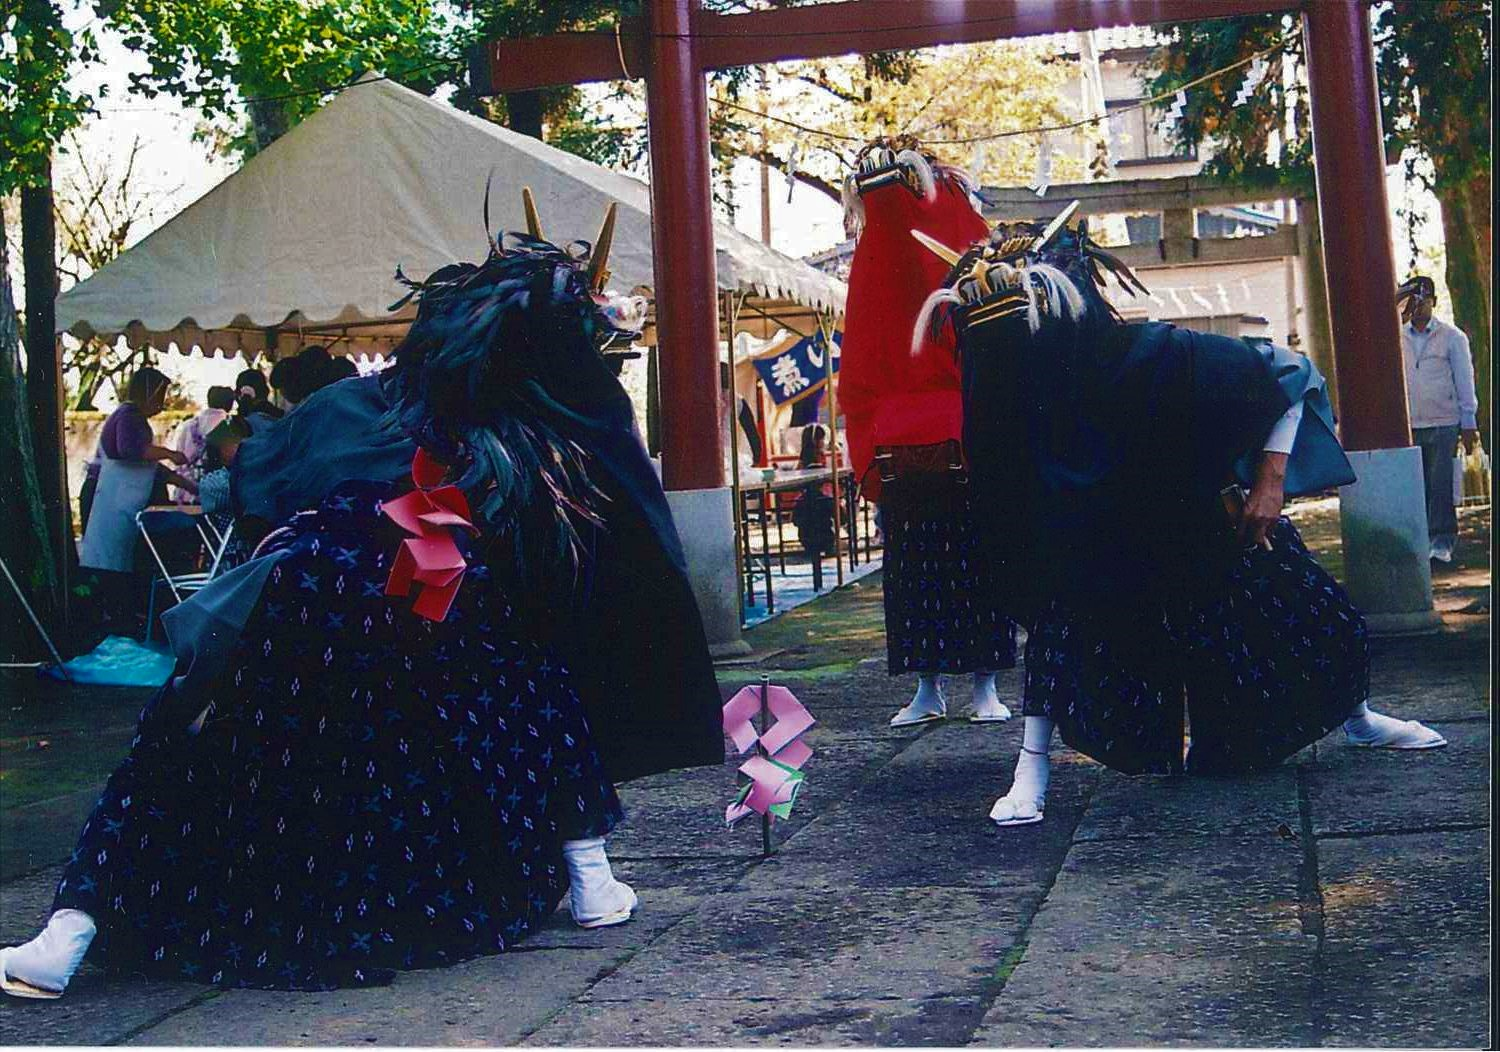
\includegraphics[clip,width=100mm]{figures/mai.jpg}
\end{center}
 \caption{ささら舞の様子 左側が後獅子 中央が女獅子 右側が前獅子}
 \label{fig:図4}
\end{figure}
地元は古くから農業を主体とする農村地帯として栄えており,女沼のささらは五穀豊穣,無病息災,天下泰平,農作物の収穫への感謝の祈りが込められている.
毎年,11月の第2日曜日に女沼地区にある女沼香取神社の秋季大祭で奉納される.
女沼のささらの期限を正確に記した文章はないが,利根川水運が最も栄えていた江戸時代に武蔵国飯積村(現埼玉県)の平井覚亮によって
伝えられたとされている.また,日光東照宮造営の際に,地固めのために招かれ,見事な舞を披露したことから,その功により
金の幣束と福草履を授けられたという伝承がある\cite{sa3}.

昔は,誰もがささらを踊れたのではなく,地区の長男に限られていた.そこから昭和に入り,戦争や核家族化によって一時衰退したが,
再興されて現在は地区に残る男子によって保存継承されている.

舞は全部で12舞あり,神に奉納する「出羽」「平庭」,物語を構成する「掛かりもの」,女獅子を争う様子を表現する「のめりこみ」などがある.現在では10舞のみ
が奉納される.





\subsection{ささら保存会と問題点}
ささら保存会は女沼のささらを保存,継承している団体である.11月の秋季大祭の他に,地元の祭りでささらを披露する.また,地元の小学生にささらを教えており,
後世に技を伝えている.

しかし,ささら保存会の人数は年々減少しており,後継者不足とささら保存会内の高齢化が問題視されている.図\ref{fig:図5}はささら保存会の人数の推移を示している.
現在は,獅子舞を披露する獅子担当10名,笛担当6名の計16名で活動している.3人1組で10舞のささら舞を獅子担当の10人で交代しながら披露するのだが,
人手不足のため,1組の踊る回数が以前と比べて増加してしまい,獅子担当の人の負担が
大きくなっている.また,1人1人,前獅子,女獅子,後獅子と役が決まっているため,役の1人でも欠けてしまうと,替えでその役を補充することが非常に難しい現状がある.



\vskip\baselineskip
\begin{figure}[h]
\begin{center}
 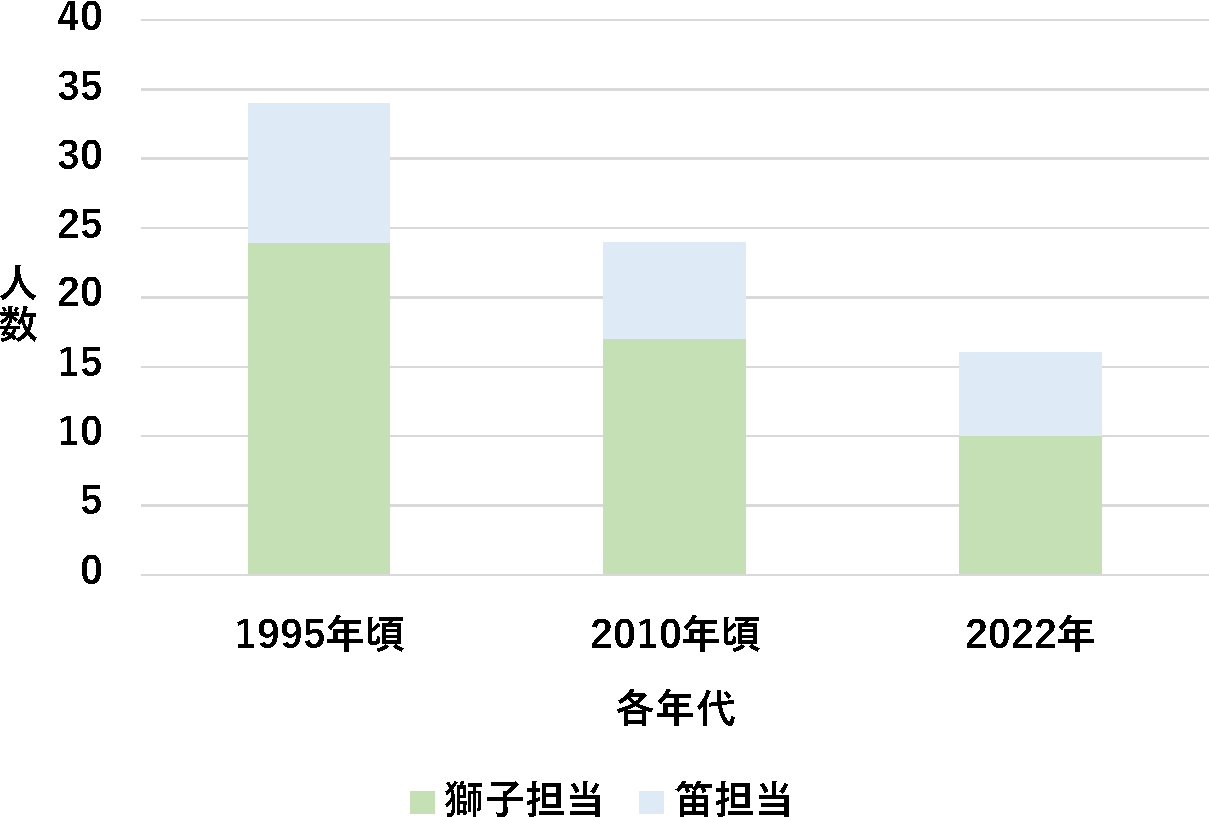
\includegraphics[clip,width=100mm]{figures/hozonkaikazu.pdf}
\end{center}
 \caption{ささら保存会の人数推移}
 \label{fig:図5}
\end{figure}


\subsection{小学生とささら}
地元の下辺見小学校では,児童が女沼のささらを披露する機会がある.児童の中には,4年生から6年生で構成される,ささら代表に参加する児童もいる.

小学校の運動会では全校生徒によるささら発表があるのだが,代表児童が中心となってささらを披露する.その際に,代表児童は,10舞ある女沼のささらの内,
「出羽」「平庭」の2幕を披露する.また,運動会の他にも地域の祭りで,小学6年生の代表児童が女沼のささら披露する機会がある.



\subsection{小学生がささらを習得する際の問題点}
ささら代表児童は,小学校の代表としてささらを踊るため,ささらの演技を立派にこなす必要がある.そのため,運動会や祭り前にささら保存会
の方々が,代表児童に数回ささらの指導を行う.

しかし,保存会の方々が代表児童にささらを教える際に問題がある.ささら保存会の人数は図\ref{fig:図5}で示した通り人数が減少しており,舞の指導を行える人が
限られてしまっている.以前は約10名で指導を行っていたが,後継者不足と仕事の都合などで,現在では3,4でしか指導を行えない状況である.そのため,代表児童
1人1人に目を向けることが難しくなり,全体に指導がいきわたらない.また,ささら保存会内の高齢化の影響で,
小学生の前でささら舞をその場で実演することが難しく,教えられる内容が限られてしまう.

上記の問題を解決するために,本研究ではささら学習教材を開発した.
\newpage
\section{開発した学習教材について}
\subsection{コンセプト}
ささら学習教材は,個人で女沼のささら舞を学習できるWeb教材である.
ささら代表児童1人1人が本教材で学習することによって,ささら保存会の負担を軽減し,
ささらを踊る上で十分な情報を得ることができる仕様となっている.本教材とささら保存会の数回の指導を
組み合わせることによって,以前より上手に踊れることを想定している.

\subsection{概要}
工夫した点は,主に良い例と悪い例の動画や写真を用いて解説し,児童に踊りのポイントを意識させて,理解しやすくした点である.

大まかに,太鼓のたたき方などの「基本」,実際に運動会で踊る「出羽」「平庭」の3つを選択できる構成とした.
この内,基本では,良い例と悪い例の動画と写真を用いて解説し,6つの踊りの動作を学習してもらう.
出羽と平庭では,はじめに正面,ななめから撮影した,踊りのポイントごとに番号が出現する踊りの通し動画を視聴してもらい,その出現した番号ごとに
良い例と悪い例の,動画と写真を用いて解説を行う.出羽は6つ,平庭は4つのポイントを解説する.
\clearpage
\subsection{サイトマップ}
本教材のサイトの構造を図\ref{fig:map}に示す.トップページには,「基本」「出羽」「平庭」3つを選択できるリンクがある.基本の画面は6つの動作,
出羽の画面は5つのポイント,平庭の画面は4つのポイントについて説明している解説ページへのリンクがある.また,出羽と平庭の画面では,斜め,正面から撮影した踊りの
通し動画が2本載っている.解説ページでは,良い例と悪い例の動画や写真を用いて説明している.

\vskip\baselineskip
\begin{figure}[h]
\begin{center}
 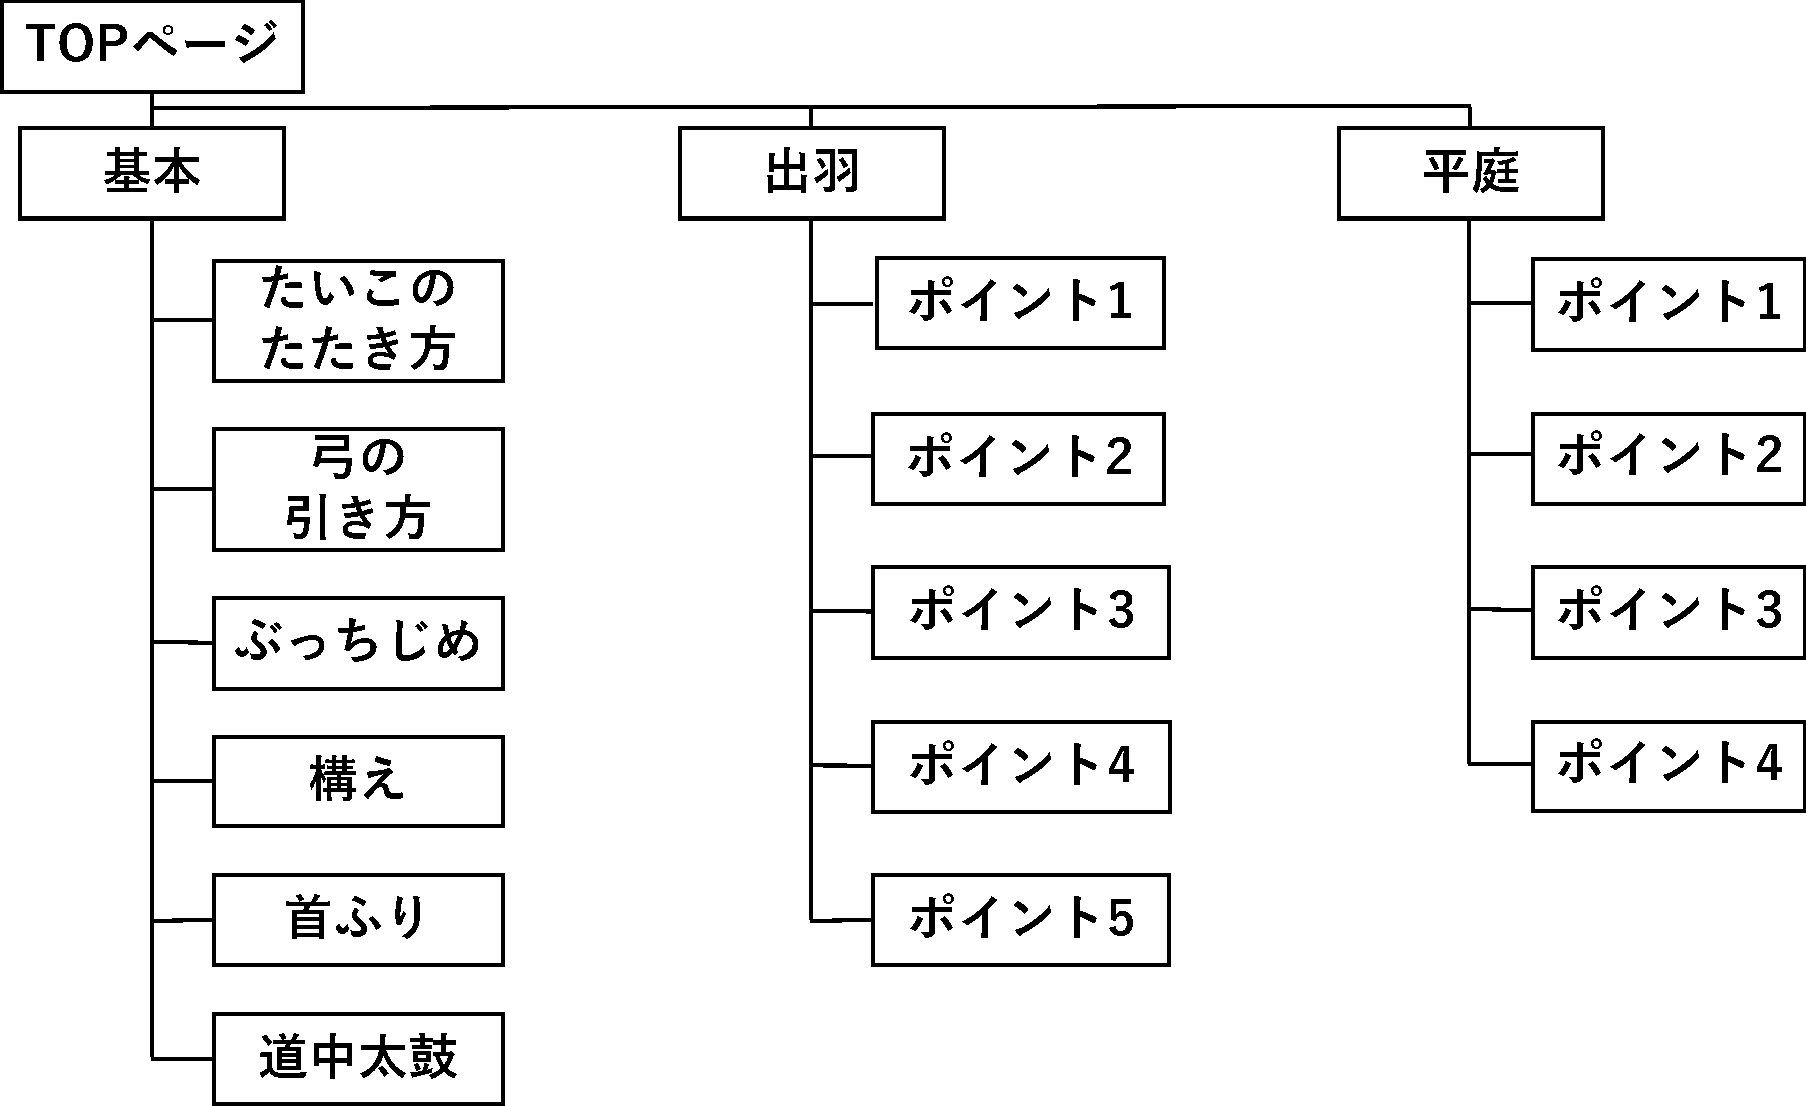
\includegraphics[clip,width=120mm]{figures/map.pdf}
\end{center}
 \caption{教材のサイトマップ}
 \label{fig:map}
\end{figure}


\clearpage
\subsection{教材で掲載している動画一覧}

基本で掲載している動画の一覧を表\ref{table:hkihon}で示す.全部で9本の動画があり,道中太鼓以外は,良い例と悪い例の動画を載せている.
道中太鼓はささらの演技前や演技後の入退場で主に太鼓をたたいて披露する踊りで,5章で説明しているささら代表児童に行ったアンケートの際に,小学生の他に在籍していた
小学校教員の方々の要望によって良い例のみ作成した.悪い例を作成しなかった理由は,図\ref{fig:map}で示した,基本の中にある「たいこのたたき方」の悪い例と
内容が重複するためである.
\begin{table}[h]
  \caption{基本の教材に掲載している動画}
  \label{table:hkihon}
  \centering
  {\renewcommand\arraystretch{2.0}
   \begin{tabular}{clll}
    \hline
    番号 & 映像タイトル & 説明 & 時間(分:秒) \\
  
    \hline \hline
    1 &  \shortstack{たいこの\\たたき方(正)} &  \shortstack{「たいこのたたき方」の\\良い例について説明している動画} & 0:19 \\
    2 &  \shortstack{たいこの\\たたき方(誤)} &  \shortstack{「たいこのたたき方」の\\悪い例について説明している動画} & 0:18 \\
    3 &  ぶっちじめ(正) &  \shortstack{ささらの基本動作である「ぶっちじめ」の\\良い例について説明している動画} & 0:33 \\
    4 & ぶっちじめ(誤) &  \shortstack{ささらの基本動作である「ぶっちじめ」の\\悪い例について説明している動画} & 0:29 \\
    5 & 構え方(正)  &  \shortstack{ささらの基本動作である「構え」の\\良い例について説明している動画} & 0:15\\
    6 & 構え方(誤) &  \shortstack{ささらの基本動作である「構え」の\\悪い例について説明している動画} & 0:19\\
    7 & 首ふり(正)  &  \shortstack{ささらの基本動作である「首ふり」の\\良い例について説明している動画} & 0:32 \\
    8 & 首ふり(誤) &  \shortstack{ささらの基本動作である「首ふり」の\\悪い例について説明している動画} & 0:32 \\
    9 & 道中太鼓 &  \shortstack{ささらの入場と退場の際に\\披露する「道中太鼓」の通し動画}& 2:39 \\

   
    \hline
   \end{tabular}
  }
 \end{table}

\clearpage

出羽で掲載している動画の一覧を表\ref{table:hdewa}に示す.全部で12本の動画があり,ポイント1からポイント5は良い例と悪い例の動画を載せている.
左斜め,正面から撮影した2本の踊りの通し動画がある理由は,1視点のみの通し動画であると,動画の中の3人の動きが重なってしまい,見ずらい箇所があるため,本教材では
2本の視点が異なる動画を提示し,満遍なく3人の動きを視聴できるようにした.

\begin{table}[h]
  \caption{出羽の教材に掲載している動画}
  \label{table:hdewa}
  \centering
  {\renewcommand\arraystretch{2.0}
   \begin{tabular}{clll}
    \hline
    番号 & 映像タイトル & 説明 & 時間(分:秒) \\
  
    \hline \hline
    1 &  左斜めから映像 &  \shortstack{出羽の通しで踊っている様子を\\左斜め前から撮影した動画} & 3:10 \\
    2 &  正面から映像 &  \shortstack{出羽の通しで踊っている様子を\\正面から撮影した動画} & 3:11 \\
    3 &  ポイント1(正) &  \shortstack{腰を下げて踊る際の\\良い例について説明している動画} & 0:27 \\
    4 &  ポイント1(誤) &  \shortstack{腰を下げて踊る際の\\悪い例について説明している動画} & 0:30 \\ 
    5 &  ポイント2(正) &  \shortstack{前獅子がバチをこすって前に進む際の\\良い例について説明している動画} & 0:08 \\ 
    6 &  ポイント2(誤) &  \shortstack{前獅子がバチをこすって前に進む際の\\悪い例について説明している動画} & 0:07 \\ 
    7 &  ポイント3(正) &  \shortstack{前獅子が弓を引きながら後ろに下がる際の\\良い例について説明している動画} & 0:26 \\ 
    8 &  ポイント3(誤) &  \shortstack{前獅子が弓を引きながら後ろに下がる際の\\悪い例について説明している動画} & 0:25 \\ 
    9 &  ポイント4(正) &  \shortstack{後獅子が前へ飛び出す際の\\良い例について説明している動画} & 0:30 \\ 
    10 &  ポイント4(誤) &  \shortstack{後獅子が前へ飛び出す際の\\悪い例について説明している動画} & 0:18 \\ 
    11 &  ポイント5(正) &  \shortstack{前獅子と後獅子が首を振りあう際の\\良い例について説明している動画} & 0:38 \\ 
    12 &  ポイント5(誤) &  \shortstack{前獅子と後獅子が首を振りあう際の\\悪い例について説明している動画} & 0:26 \\ 




  

    \hline
   \end{tabular}
  }
 \end{table}
 
 \clearpage

 平庭で掲載している動画の一覧を表\ref{table:hhiraniwa}に示す.全部で10本の動画があり,ポイント1からポイント4は良い例と悪い例の動画を載せている.そして,
 出羽と同様に,左斜め,正面から撮影した2本の踊りの通し動画がある.
 
 \begin{table}[h]
   \caption{平庭の教材に掲載している動画}
   \label{table:hhiraniwa}
   \centering
   {\renewcommand\arraystretch{2.0}
    \begin{tabular}{clll}
     \hline
     番号 & 映像タイトル & 説明 & 時間(分:秒) \\
   
     \hline \hline
     1 &  左斜めから映像 &  \shortstack{平庭の通しで踊っている様子を\\左斜め前から撮影した動画} & 5:14 \\
     2 &  正面から映像 &  \shortstack{平庭の通しで踊っている様子を\\正面から撮影した動画} & 5:13 \\
     3 &  ポイント1(正) &  \shortstack{足踏みをする際の\\良い例について説明している動画} & 0:21 \\
     4 &  ポイント1(誤) &  \shortstack{足踏みをする際の\\悪い例について説明している動画} & 0:24 \\ 
     5 &  ポイント2(正) &  \shortstack{3人が同時に回る際の\\良い例について説明している動画} & 0:52 \\ 
     6 &  ポイント2(誤) &  \shortstack{3人が同時に回る際の\\悪い例について説明している動画} & 0:48 \\ 
     7 &  ポイント3(正) &  \shortstack{弓を引いた後にぶっちじめをする際の\\良い例について説明している動画} & 0:33 \\ 
     8 &  ポイント3(誤) &  \shortstack{弓を引いた後にぶっちじめをする際の\\悪い例について説明している動画} & 0:32 \\ 
     9 &  ポイント4(正) &  \shortstack{回り終わって足踏みをする際の\\良い例について説明している動画} & 0:50 \\ 
     10 &  ポイント4(誤) &  \shortstack{回り終わって足踏みをする際の\\悪い例について説明している動画} & 0:46 \\ 
   
 
 
 
 
   
 
     \hline
    \end{tabular}
   }
  \end{table}
 


\clearpage
\subsection{使い方}
図\ref{fig:map}で示した,本教材のトップページでは上段に画面の説明を,中段に「基本」「出羽」「平庭」の3つを選択できるリンクを提示するようにした.学習者は
自分の学習したい項目を選択することが可能である.トップページの画面を図\ref{fig:top}に示す.
\vskip\baselineskip
\begin{figure}[h]
\begin{center}
 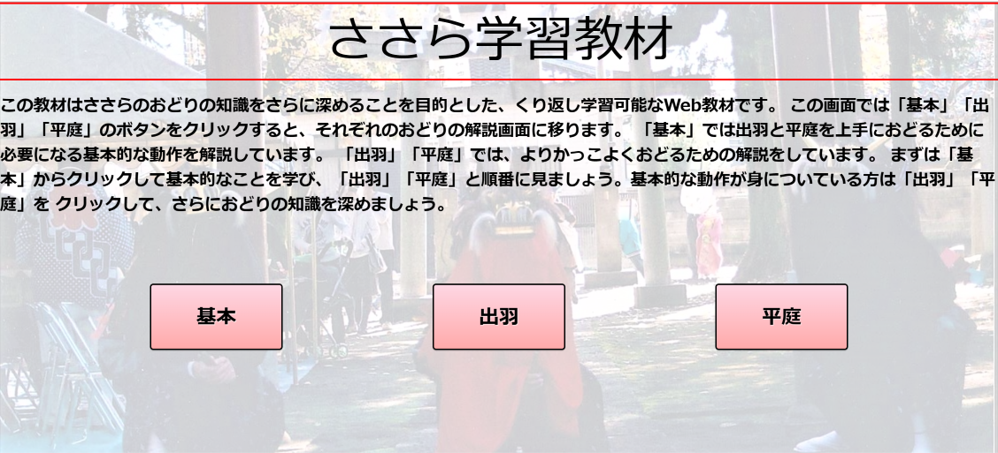
\includegraphics[clip,width=100mm]{figures/top.png}
\end{center}
 \caption{ささら学習教材トップページ}
 \label{fig:top}
\end{figure}

基本では,ささらを上手に踊るために必要な6つの動作を学習してもらう.ここで学習する内容は出羽や平庭にも通じており,主に初級者向けの内容となっている.
基本の画面を図\ref{fig:kihontop}に示す.上段に画面の説明を,中段に6つの動作を選択できるリンクを提示するようにした.内容は左から「太鼓のたたき方」
「弓の引き方」「ぶっちじめ」「構え」「首ふり」「道中太鼓」となっている.
\vskip\baselineskip
\begin{figure}[h]
\begin{center}
  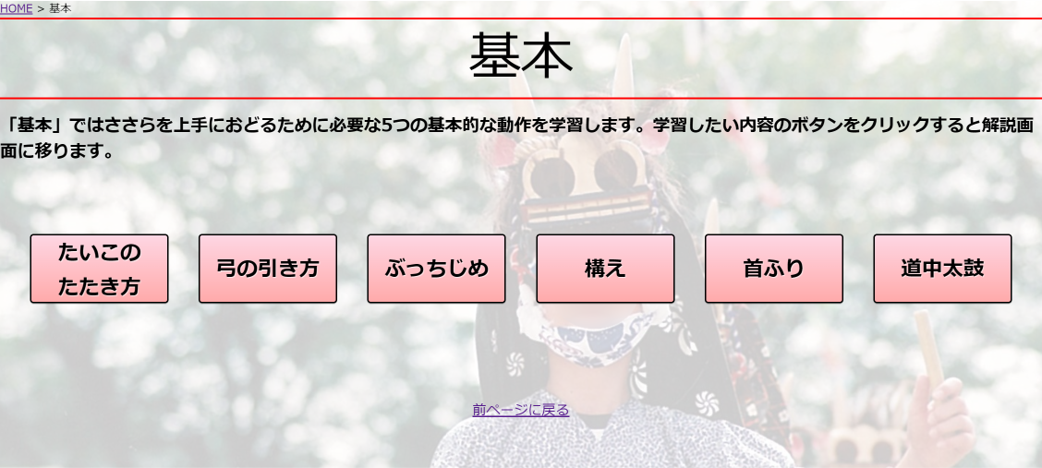
\includegraphics[clip,width=100mm]{figures/kihontop.png}
\end{center}
 \caption{基本画面}
 \label{fig:kihontop}
\end{figure}
\noindent
例として,太鼓のたたき方を選択した画面を図\ref{fig:kihon2}に示す.
上段に説明文を,中段左に良い例の映像を,中段右に悪い例の映像を,下段に学習者に注目してほしい点を提示している.
\vskip\baselineskip
\begin{figure}[h]
\begin{center}
  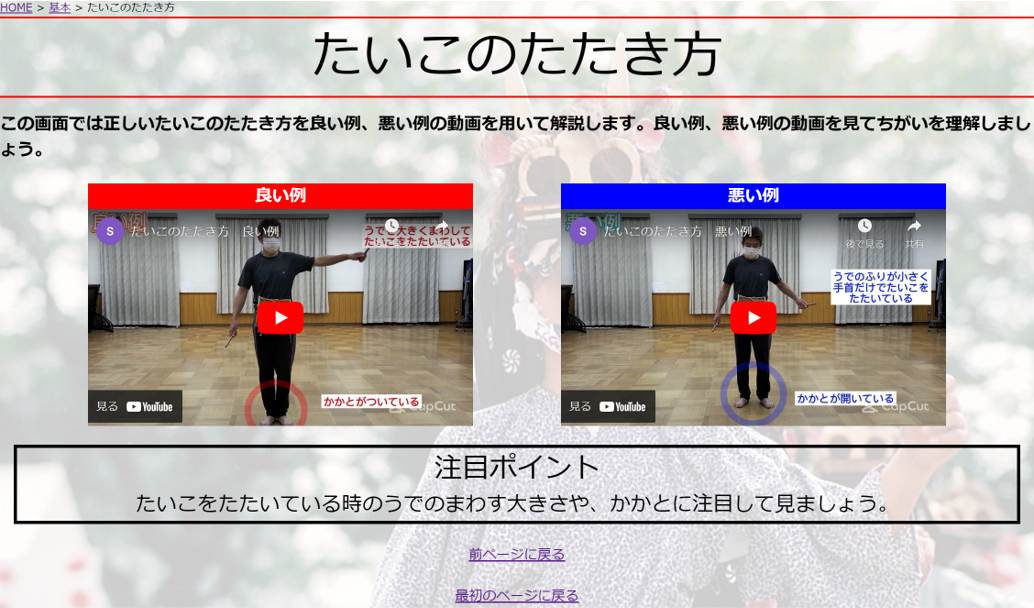
\includegraphics[clip,width=100mm]{figures/kihon2.png}
\end{center}
 \caption{たいこのたたき方の解説ページ}
 \label{fig:kihon2}
\end{figure}

\newpage

図\ref{fig:map}で示した出羽では,代表児童が間違えて覚えてしまっている動作を中心に,ささら保存会の方が毎年教えているポイントを学習してもらう.
出羽の画面を図\ref{fig:dewatop}に示す.上段に画面の説明を,中段左に斜めから撮影した通し動画を,中段右に正面から撮影した通し動画を,下段に踊りのポイント
番号を提示している.

\vskip\baselineskip
\begin{figure}[h]
\begin{center}
  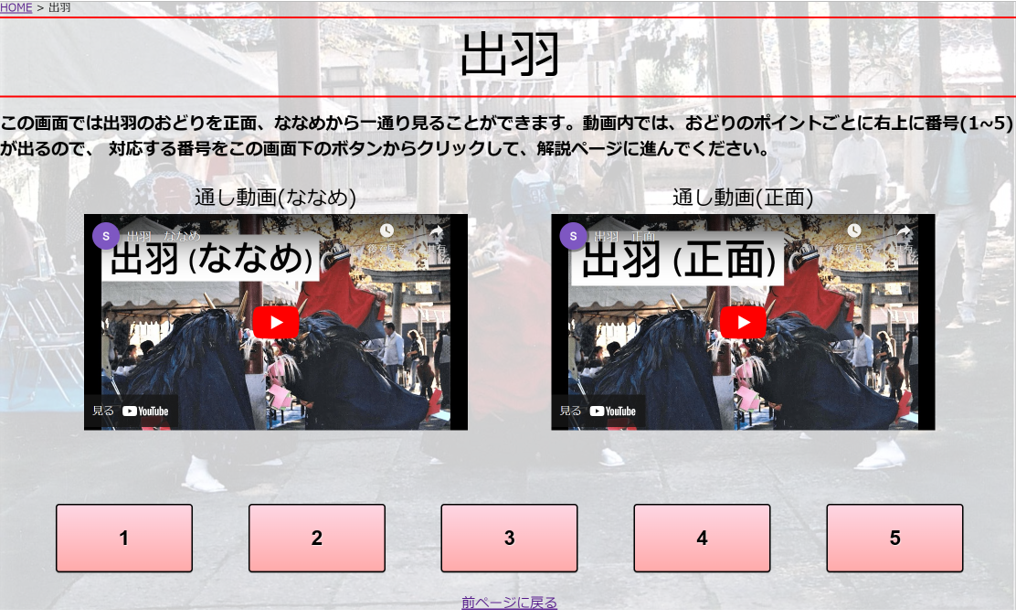
\includegraphics[clip,width=100mm]{figures/dewatop.png}
\end{center}
 \caption{出羽画面}
 \label{fig:dewatop}
\end{figure}
\noindent
ポイント番号については,斜め,正面から撮影した通し動画を視聴すると,図\ref{fig:dewa2}のように,動画内でポイントごとに右上に番号が出現するようになっているため,その対応する
ポイント番号をクリックすると,ポイントの解説ページに遷移する.
\vskip\baselineskip
\begin{figure}[h]
\begin{center}
  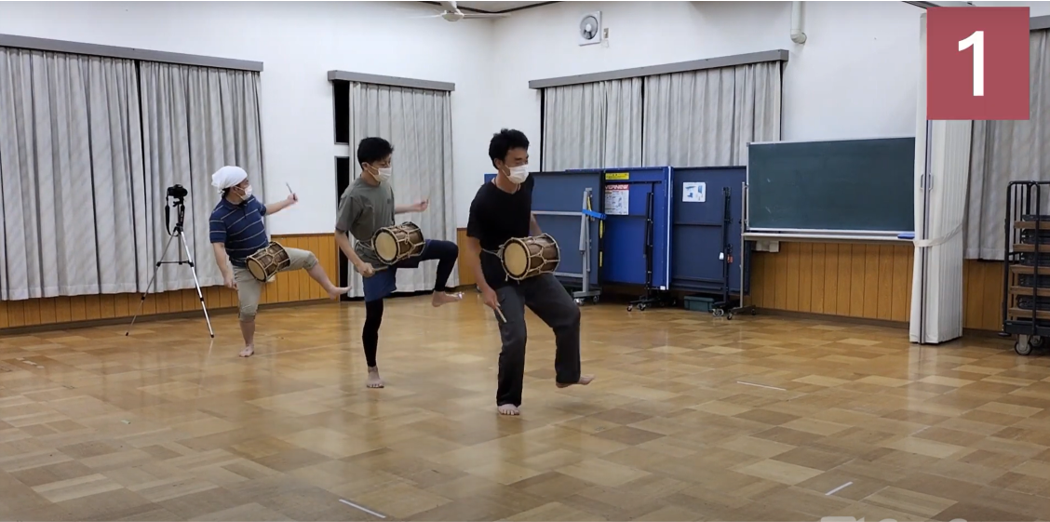
\includegraphics[clip,width=100mm]{figures/dewa2.png}
\end{center}
 \caption{出羽 斜めから撮影した通し動画}
 \label{fig:dewa2}
\end{figure}
\noindent
例として,ポイント番号1を選択し,遷移した画面を図\ref{fig:dewa3}に示す.基本のたいこのたたき方を選択した画面と構成は同じである.

平庭は出羽と操作方法が同じなため,省略する.

\vskip\baselineskip
\begin{figure}[h]
\begin{center}
  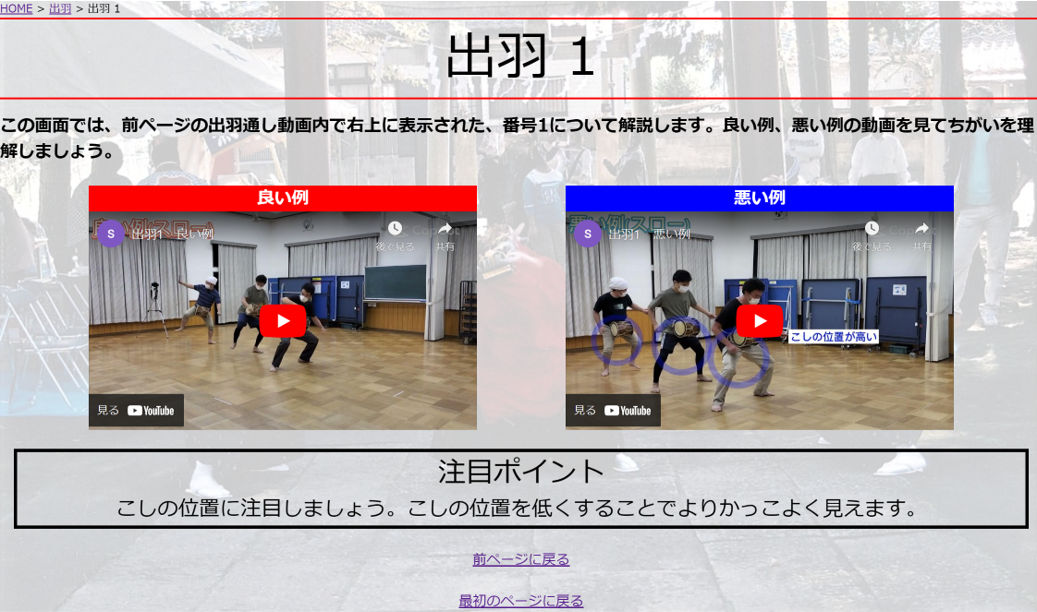
\includegraphics[clip,width=100mm]{figures/dewa3.png}
\end{center}
 \caption{出羽 ポイント番号1の解説ページ}
 \label{fig:dewa3}
\end{figure}

\clearpage
\section{学習教材の評価}
\subsection{アンケート調査}

本教材の有用性を示すために,アンケート調査を実施した.
\subsubsection{アンケート対象者}
アンケート対象者は,地元小学校のささら代表児童5名である.地元の祭り前の,ささら代表児童とささら保存会の2回の合同練習に参加させて
頂き,ささら保存会の方々の協力の元,実施した.

5名のささら代表歴は図\ref{fig:an1}となっており,アンケートの項目1で調査した.4年生からささらの代表になった児童は
2人,5年生からささらの代表になった児童は3人,6年生からささらの代表になった児童は0人という結果だった.このことから,今回調査を行ったささら代表児童は,
すでにささら保存会の方々の指導を受けており,ある程度,ささらの踊りの知識がある児童ということになる.

\vskip\baselineskip
\begin{figure}[h]
\begin{center}
  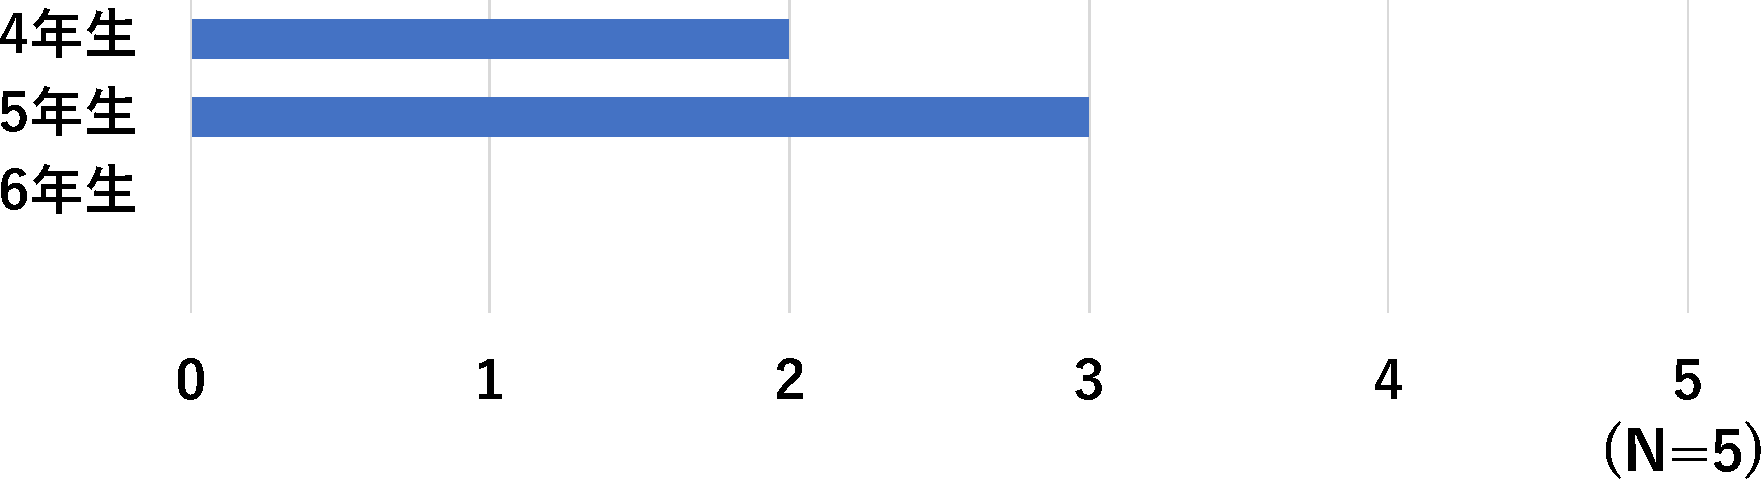
\includegraphics[clip,width=100mm]{figures/anket/an1.pdf}
\end{center}
 \caption{ささら代表児童に何年生の時になりましたか}
 \label{fig:an1}
\end{figure}
\noindent

\subsubsection{アンケ―トの形式}
1回目の練習時に,ささら学習教材の説明をし,アンケートを用紙を配布した.1週間後の2回目の練習時に回収した.各項目に対して,「とてもそう思う」「そう思う」
「そう思わない」「全くそう思わない」の4つの選択肢から1つ回答してもらった.

\subsubsection{アンケートの内容}
アンケートの項目は全部で9つある.
ささら代表歴についての項目以外は,大きく分けて,
教材の使いやすさ,教材の工夫した点の評価,実用的の3つに分けられる.






\subsection{アンケートの目的}
大きく3つに分けた項目の目的を以下で説明する.
\subsubsection{教材の使いやすさについての項目}
本教材は,利用するささら代表児童の年齢層に合わせて作成し,漢字なども極力使用しなかった.「トップページ」のような小学生にとって馴染みのない言葉は,
「最初のページ」と表現し,小学生がスムーズに操作できるように心掛けた.また,利用するデバイスによって画面の大きさが異なるため,
スマ―トフォンの縦画面,横画面,パソコン画面に合わせてUIを設計した.図\ref{fig:dewa3}はパソコンで視聴した際の画面で,同じ画面をスマ―トフォンの縦画面と横画面に
した際の様子を図\ref{fig:tate},\ref{fig:yoko}に示す.
\vskip\baselineskip
\begin{figure}[h]
\begin{center}
  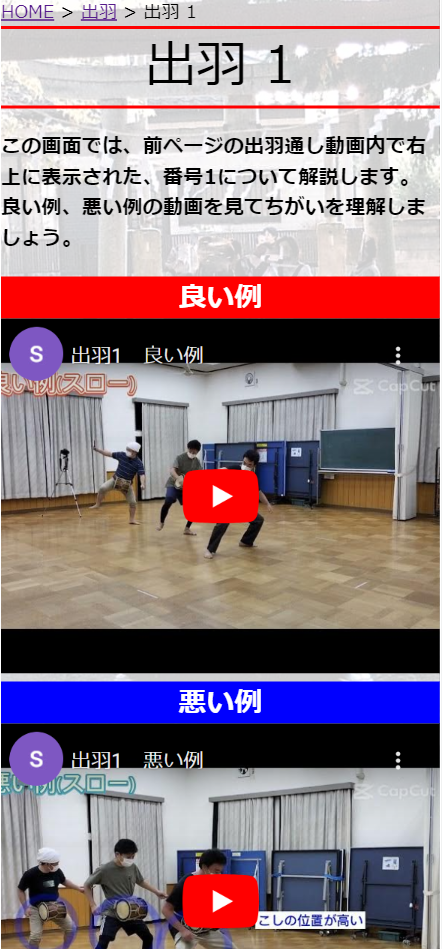
\includegraphics[clip,width=50mm]{figures/tate.png}
\end{center}
 \caption{スマ―トフォンの縦画面}
 \label{fig:tate}
\end{figure}
\newpage
\vskip\baselineskip
\begin{figure}[t]
\begin{center}
  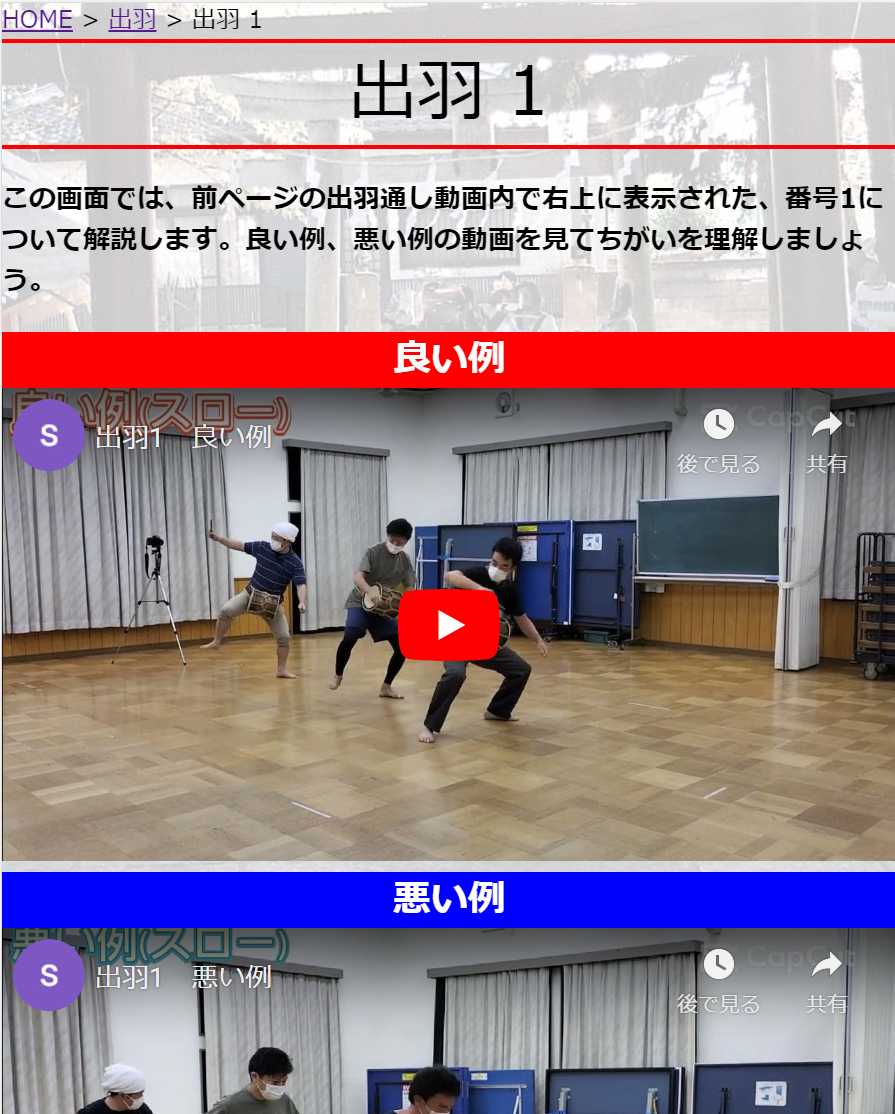
\includegraphics[clip,width=70mm]{figures/yoko.png}
\end{center}
 \caption{スマ―トフォンの横画面}
 \label{fig:yoko}
\end{figure}


ささら学習教材は,個人で学習を進めることを想定している.そのため,この項目の目的は,上記の考慮して設計した点を踏まえて,ささら代表児童が問題なく
本教材を操作することができ,個人で学習を進めることが可能かを調査するためである.


\subsubsection{工夫した点についての項目}
ささら代表児童に十分な踊りの情報を提供する為に工夫した点は,良い例と悪い例の動画や写真を用いて解説することで,ささら代表児童に踊りのポイントを
意識させて,理解しやすくした点である.動画内では,図\ref{fig:kosinoiti}のように,体の1部を丸で囲むなどして,学習者に注目してほしいポイントを明白にした.
また,ささら舞の動作は早いため,通常再生だと,学習者が踊りの動きをよく確認できない.そこで,早い動きにはスロー再生を用いて,わかりやすく解説するようにした.
\vskip\baselineskip
\begin{figure}[h]
\begin{center}
  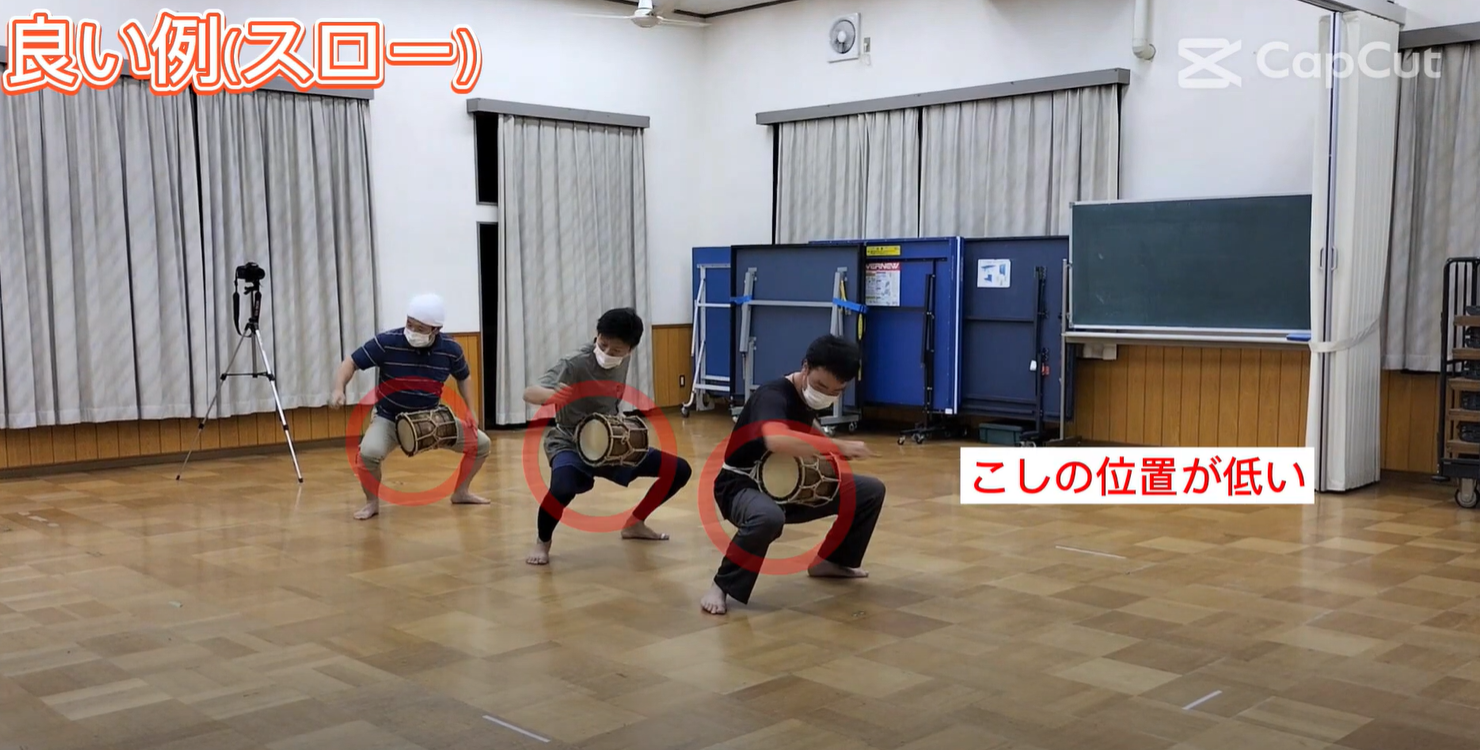
\includegraphics[clip,width=100mm]{figures/kosinoiti.png}
\end{center}
 \caption{動画内で腰の位置に丸をつけて解説している画面}
 \label{fig:kosinoiti}
\end{figure}

上記の工夫した点を踏まえて,この項目の目的は,工夫した点によって,ささら代表児童が踊りの情報を十分に得ることが可能かを調査するためである.

\subsubsection{実用的についての項目}
本教材は最終的に,ささら保存会の数回の指導と組み合わせることで,ささら代表児童がさらに上手に踊れることを目標としている.そのため,この項目
の目的は,代表児童にとって,ささら学習教材が実用的かを調査するためである.
\clearpage
\subsection{アンケート結果と考察}
アンケート結果と考察について記述する.
\subsubsection{教材の使いやすさについての項目}
教材の使いやすさについては4項目ある.
\vskip\baselineskip
\begin{figure}[h]
\begin{center}
  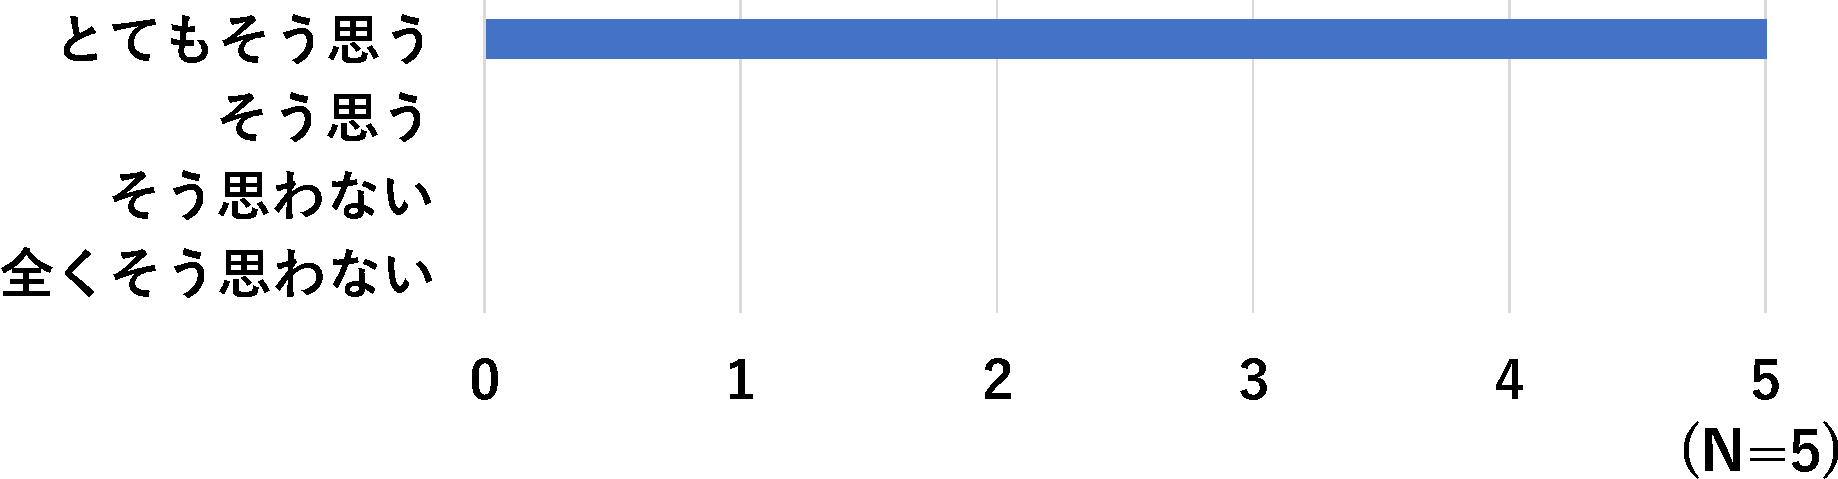
\includegraphics[clip,width=100mm]{figures/anket/an2.pdf}
\end{center}
 \caption{ささら学習教材は使いやすかったですか}
 \label{fig:an2}
\end{figure}

図\ref{fig:an2}の項目では,5人全員が「とてもそう思う」を選択した.
\vskip\baselineskip
\begin{figure}[h]
\begin{center}
  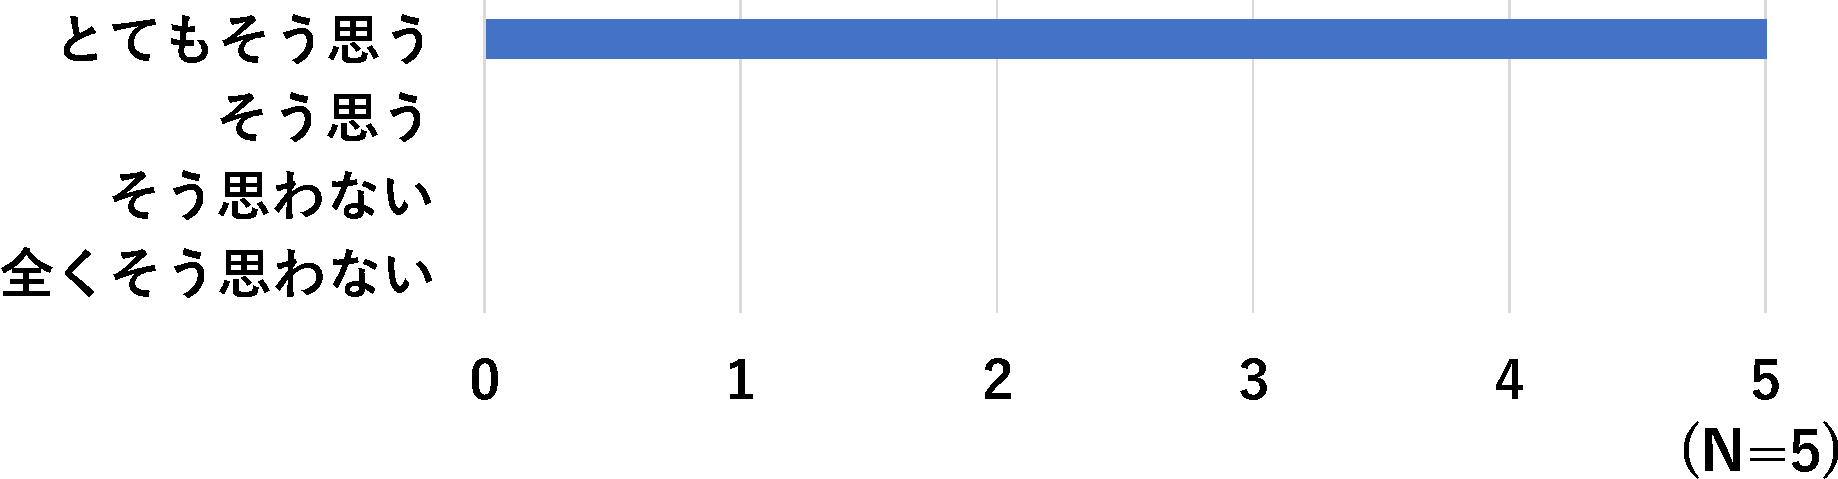
\includegraphics[clip,width=100mm]{figures/anket/an3.pdf}
\end{center}
 \caption{自分の見たいページにたどり着くことができましたか}
 \label{fig:an3}
\end{figure}

図\ref{fig:an3}の項目では,5人全員が「とてもそう思う」を選択した.

\vskip\baselineskip
\begin{figure}[h]
  \begin{center}
    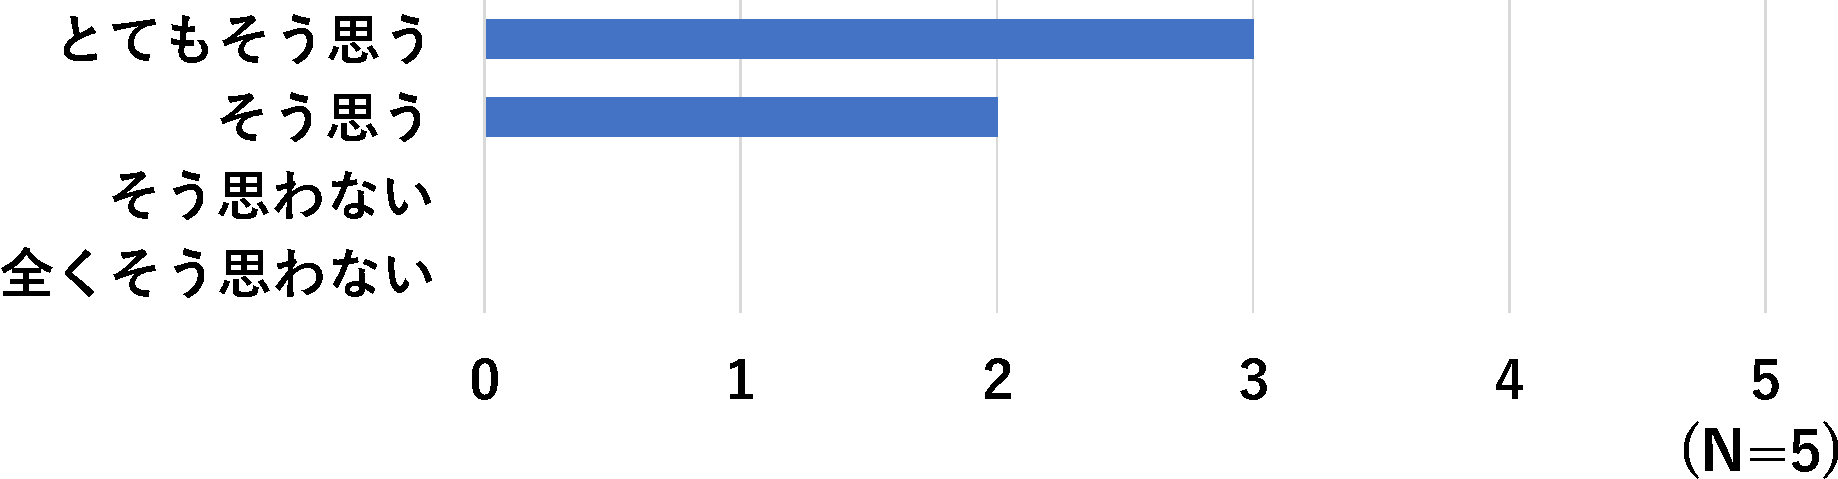
\includegraphics[clip,width=100mm]{figures/anket/an4.pdf}
  \end{center}
   \caption{1人でささら学習教材を用いてささらのおどりを学習することができましたか}
   \label{fig:an4}
  \end{figure}

  図\ref{fig:an4}の項目では,3人が「とてもそう思う」2人が「そう思う」を選択した.

\vskip\baselineskip
\begin{figure}[h]
\begin{center}
  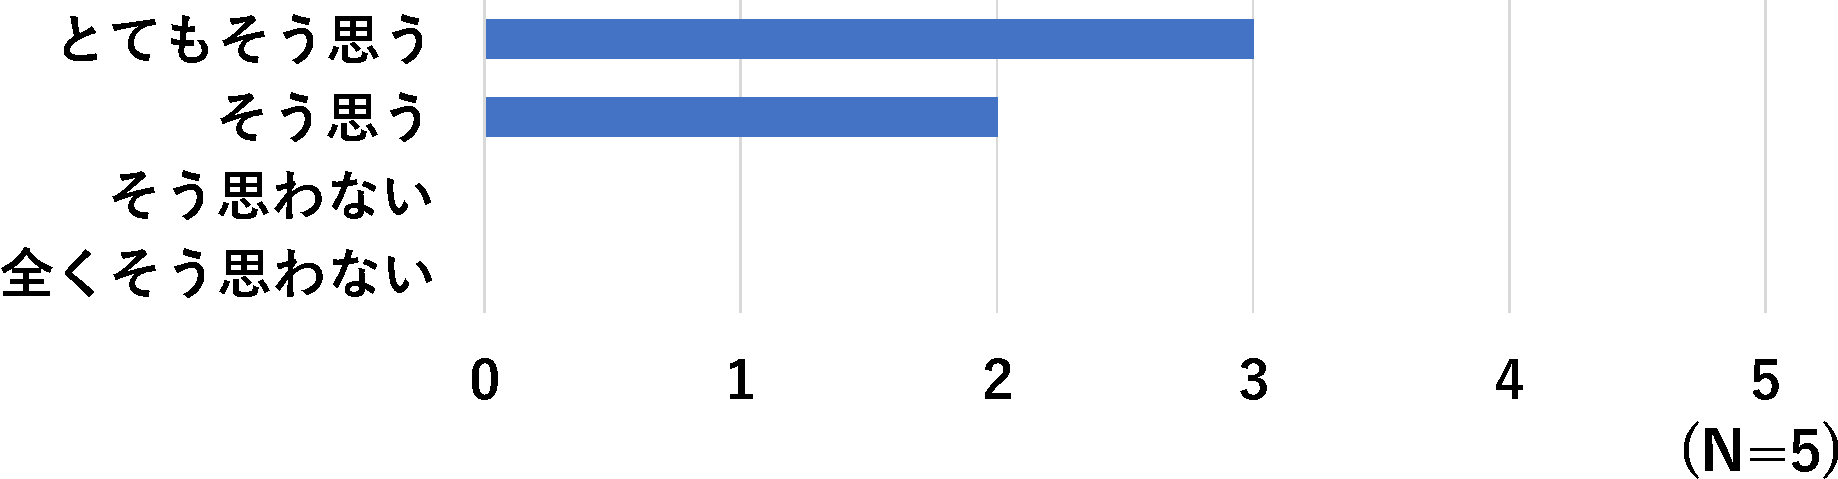
\includegraphics[clip,width=100mm]{figures/anket/an7.pdf}
\end{center}
 \caption{ボタンの大きさや文字の大きさは適切でしたか}
 \label{fig:an7}
\end{figure}

図\ref{fig:an7}の項目では,3人が「とてもそう思う」2人が「そう思う」を選択した.



上記の4つの結果が高評価なことから,本教材がささら代表児童にとって利便性があり,個人でささらの踊りの学習を進めることが可能であると
考える.

\subsubsection{工夫した点の評価についての項目}
工夫した点の評価については2項目ある.
\vskip\baselineskip
\begin{figure}[h]
\begin{center}
  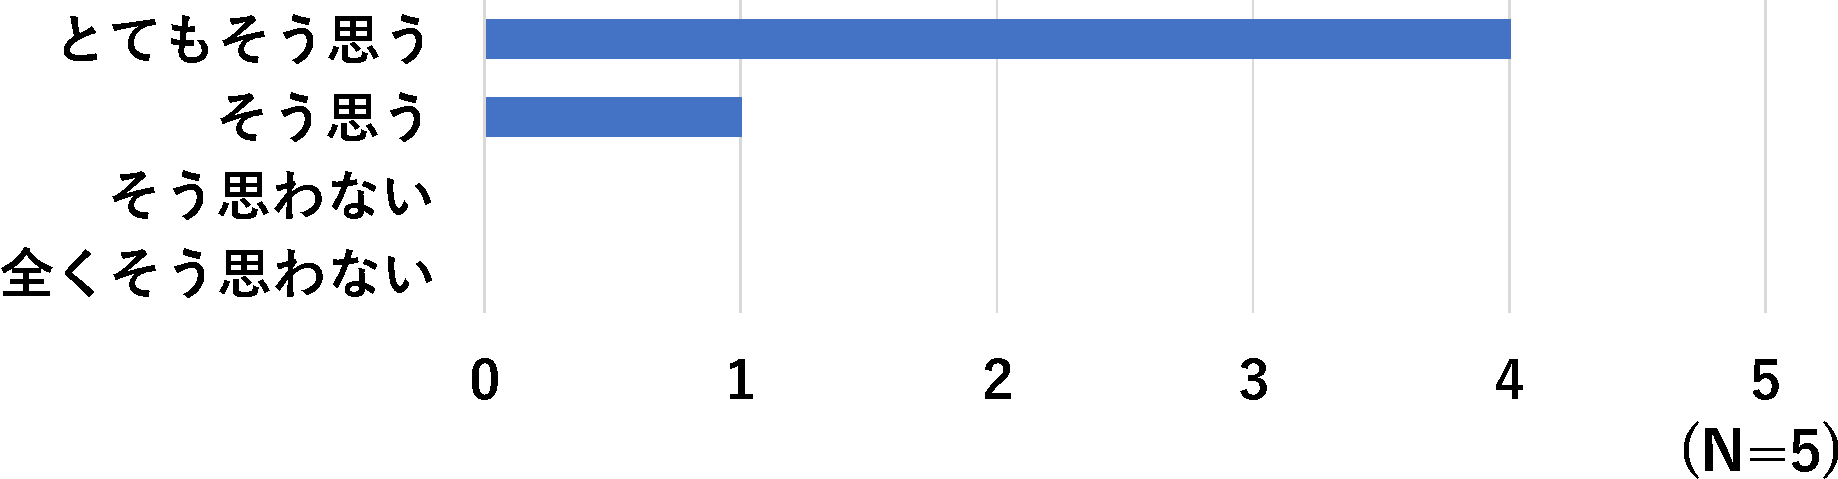
\includegraphics[clip,width=100mm]{figures/anket/an5.pdf}
\end{center}
 \caption{良い例と悪い例の動画や写真を見比べて,自分のまちがいに気づくことができましたか}
 \label{fig:an5}
\end{figure}
図\ref{fig:an5}より,4人が「とてもそう思う」1人が「そう思う」を選択した.

\vskip\baselineskip
\begin{figure}[h]
\begin{center}
  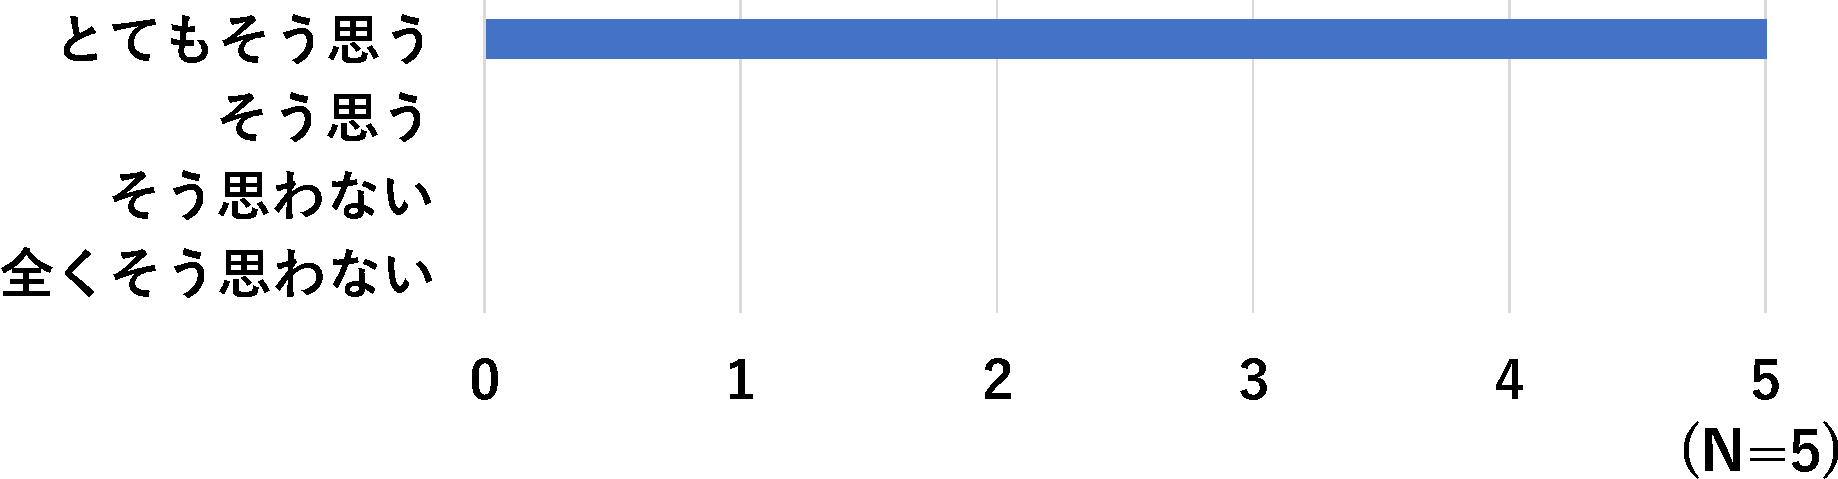
\includegraphics[clip,width=100mm]{figures/anket/an6.pdf}
\end{center}
 \caption{良い例と悪い例を用いて解説しているページで,十分なおどりの情報を得ることができましたか}
 \label{fig:an6}
\end{figure}

図\ref{fig:an6}より,5人が「とてもそう思う」を選択した.

上記の2つの結果が高評価なことから,良い例と悪い例の動画や写真を用いて,動きのポイントを
分かりやすくすることによって,十分な踊りの知識を提供できることが分かる.
\newpage
\subsubsection{実用的についての項目}
実用的については2項目ある.

\vskip\baselineskip
\begin{figure}[h]
\begin{center}
  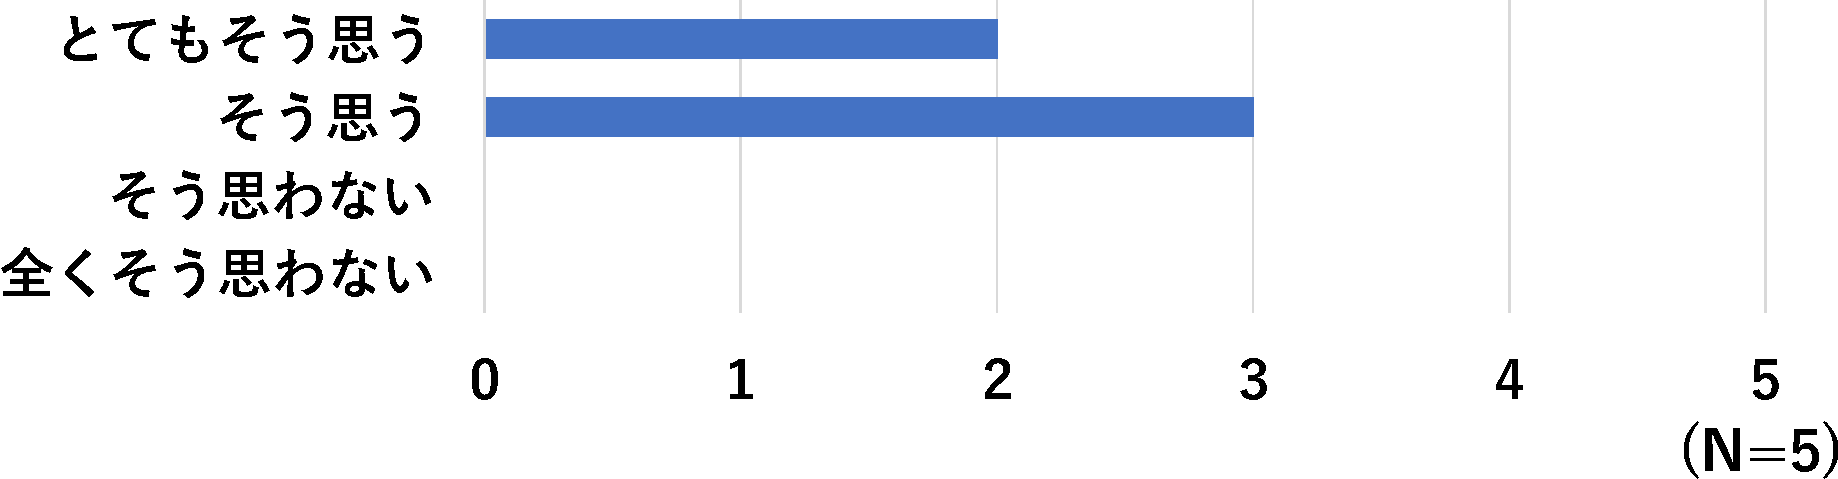
\includegraphics[clip,width=100mm]{figures/anket/an8.pdf}
\end{center}
 \caption{ささら保存会の,年に数回(運動会前や祭りの前)だけでささらを上手におどれると思いますか}
 \label{fig:an8}
\end{figure}

図\ref{fig:an8}より,2人が「とてもそう思う」3人が「そう思う」を選択した.

図\ref{fig:an8}は,低評価が多くなると想定していたが,結果から,ささら代表児童にとって数回のささら保存会の指導だけで
満足していることが分かる.しかし,ささら保存会の方々は,代表児童1人1人に対して満足な指導を行えてないと発言
している.そのため,ささら代表児童は,ささら保存会の十分とは言えない指導で満足しているため,
踊りの技術がさらに上達しない可能性があると考える.

\vskip\baselineskip
\begin{figure}[h]
\begin{center}
  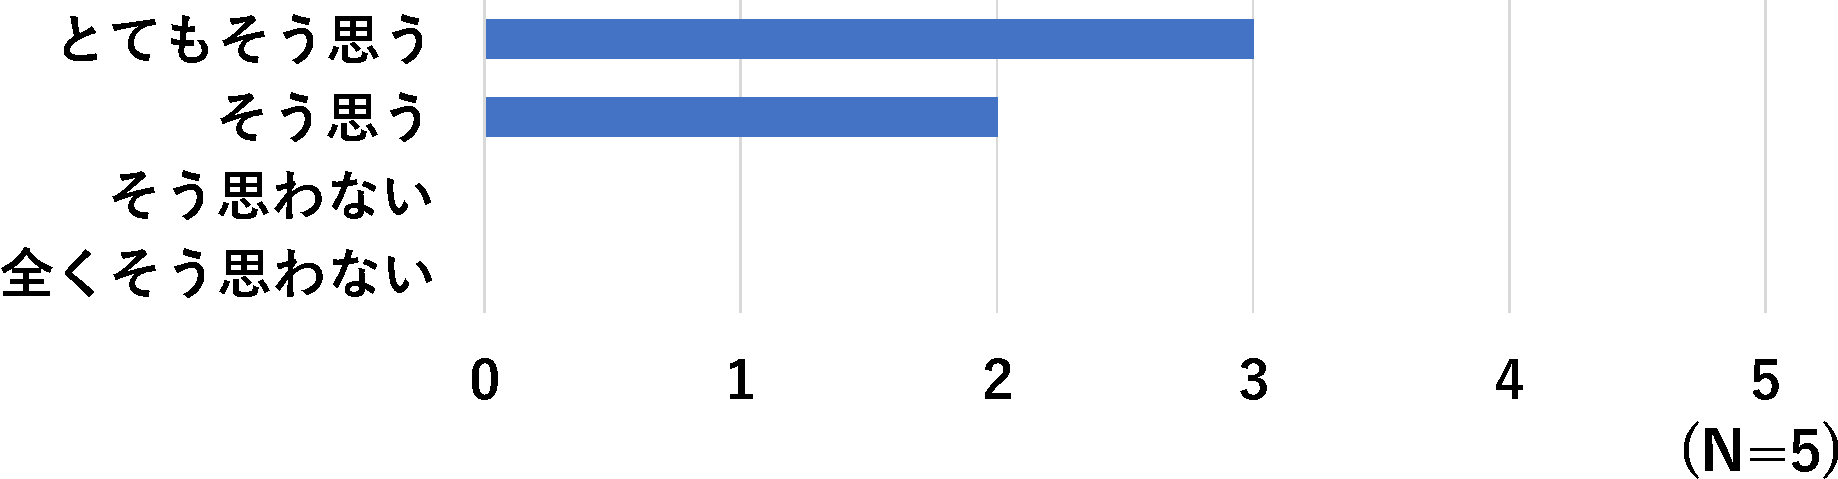
\includegraphics[clip,width=100mm]{figures/anket/an9.pdf}
\end{center}
 \caption{ささら保存会の教えと,ささら学習教材を組み合わせれば今までより上手におどれると思いますか}
 \label{fig:an9}
\end{figure}
図\ref{fig:an9}より,3人が「とてもそう思う」2人が「そう思う」を選択した.



図\ref{fig:an9}の結果が高評価なことから,本教材の実用性を示すことができた.








\newpage
\section{結言}
%背景

本研究では,民俗芸能の女沼のささらが抱えている育成問題を解決するために,
ビデオ教材を開発した.

6年生のささら代表児童5名に対してのアンケートは大きく3つに分かれており,「教材の使いやすさ」,「教材の工夫した点の評価」,「実用的」について調査を行った.
「教材の使いやすさ」が高評価なことから,本教材は利便性が高く,問題なく個人で学習を進められることが分かった.
「教材の工夫した点の評価」が高評価なことから,良い例と悪い例の動画や写真を用いて,動きのポイントを
分かりやすくすることによって,十分な踊りの知識を提供できることが分かった.
「実用的」が高評価なことから,本教材と数回のささら保存会の指導を組み合わせることで,以前よりも踊りの技術を向上させれることが分かった.
上記のことから,本研究の目的を達成し,教材の有用性を確かめることができた.

地元の民俗芸能が,高齢化と後継者不足によって満足に指導することができない状況なので,全国の主要な伝統芸能も同じ
育成問題を抱えていると考える.そこで,本教材のような,良い例と悪い例を用いて解説しているビデオ教材を作成することで
解決への糸口になると考える.



\newpage
\section{謝辞}
本研究の遂行及び本論文の作成にあたり,須田研究室の仲間とささら保存会の方々に多くの手助けを頂きました,深く感謝の意を表します.そして,本論文の作成にあたり
多大なる御指導及び御助言を頂きました,須田宇宙准教授に深く感謝の意を表します.
\newpage
\addcontentsline{toc}{section}{参考文献}
\begin{thebibliography}{99}
\bibitem{kabuki} 小野和俊 「学校百科・はじめてみる伝統芸能1 歌舞伎」,クロスロード,1989年3月25日第一刷
\bibitem{nou} 小野和俊 「学校百科・はじめてみる伝統芸能2 能・狂言」,クロスロード,1989年3月25日第一刷
\bibitem{bun} 小野和俊 「学校百科・はじめてみる伝統芸能3 文楽」,クロスロード,1989年3月25日第一刷
\bibitem{koten} 小野和俊 「学校百科・はじめてみる伝統芸能4 古典落語」,クロスロード,1989年3月25日第一刷
\bibitem{kamon} 読売新聞オンライン : ``伝統芸能 次代の担い手を確保したい'', \url{https://www.yomiuri.co.jp/editorial/20220515-OYT1T50201/}, 2023/1/1 参照
\bibitem{sa2} Iwanichi Online 岩手日日新聞社: ``民俗芸能団体運営課題 「後継者不足」最多 北上市連合会 伝承の維持厳しく'', \url{https://www.iwanichi.co.jp/2018/11/05/250225/}, 2023/1/1 参照
\bibitem{sa3} 古河市 生涯学習課: ``女沼のささら(市指定文化財)/古河市公式ホームページ'', \url{https://www.city.ibaraki-koga.lg.jp/soshiki/syogaigakusyu/15/2403.html}, 2022/8/8 参照



\end{thebibliography}





\end{document}


